\subsubsection{Sample size (Surrogate size) 10*10 }
In this section we calculated flamespeed values for 100 (10*10) different points in the domain and the remaining values are linear combination of these 100 points.  The results below are for sample size $1e5$, $5e5$ , $1e6$, $5e6$ and $1e7$. 

\begin{figure}[H]
\centering
\subfloat[MCMC raw chain of samples of $E_2$\label{subfig-1:dummy}]{%
     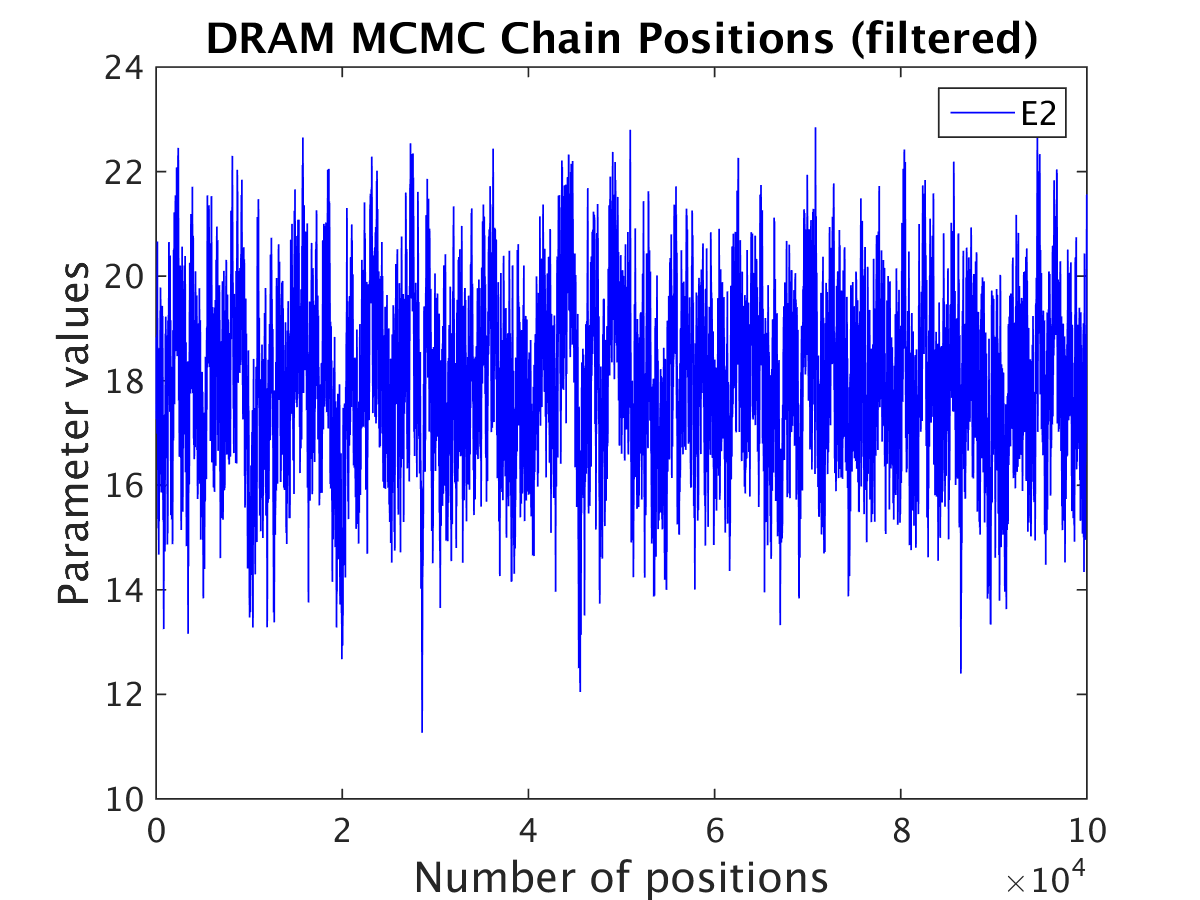
\includegraphics[scale=0.7]{multiple_data/10_kde/outputData_1e5/simple_ip_chain_pos_raw_1} 
    }
    \quad
    \subfloat[MCMC raw chain of samples of $E_2$\label{subfig-1:dummy}]{%
         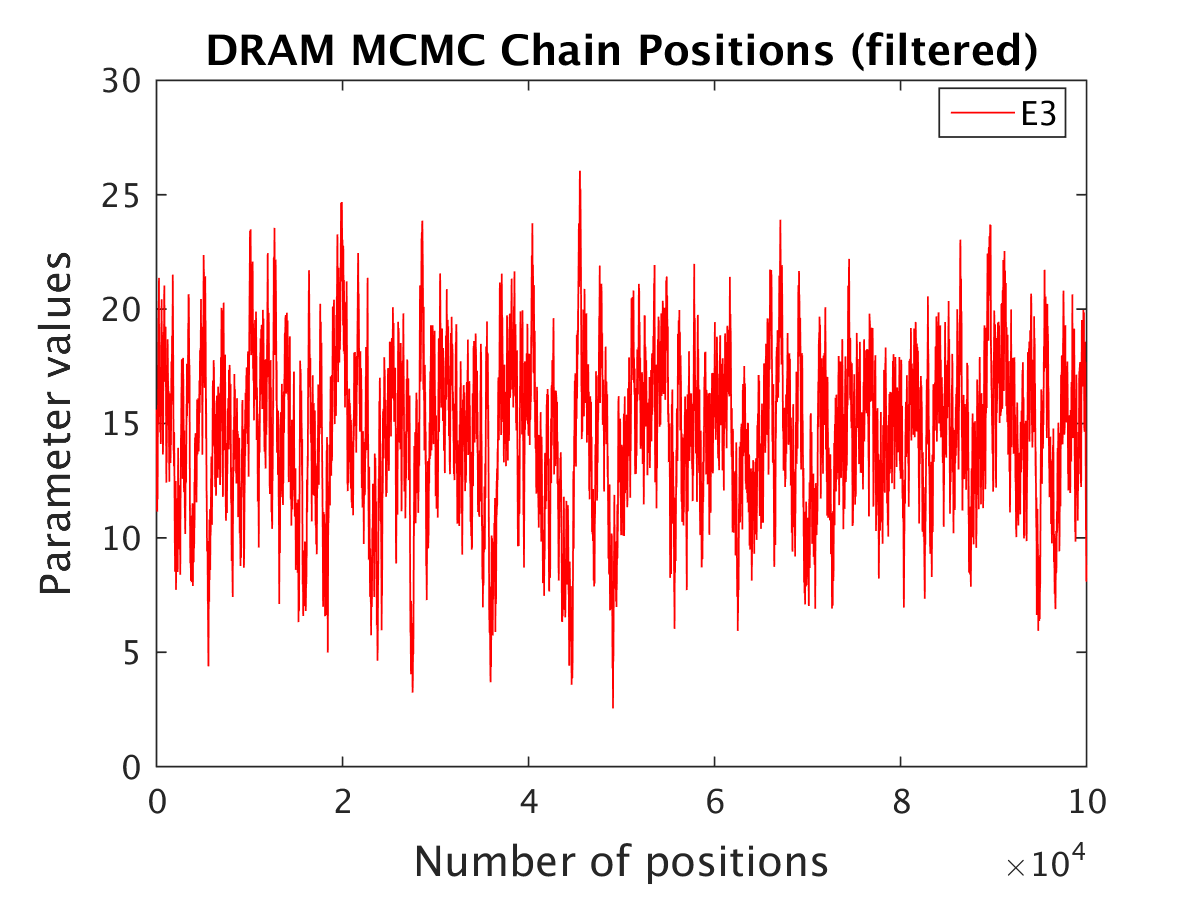
\includegraphics[scale=0.7]{multiple_data/10_kde/outputData_1e5/simple_ip_chain_pos_raw_2} 
        }
    \end{figure}
  \begin{figure}[H]
  \ContinuedFloat
  \centering
  \subfloat[Histogram for $E_2$ \label{subfig-1:dummy}]{%
       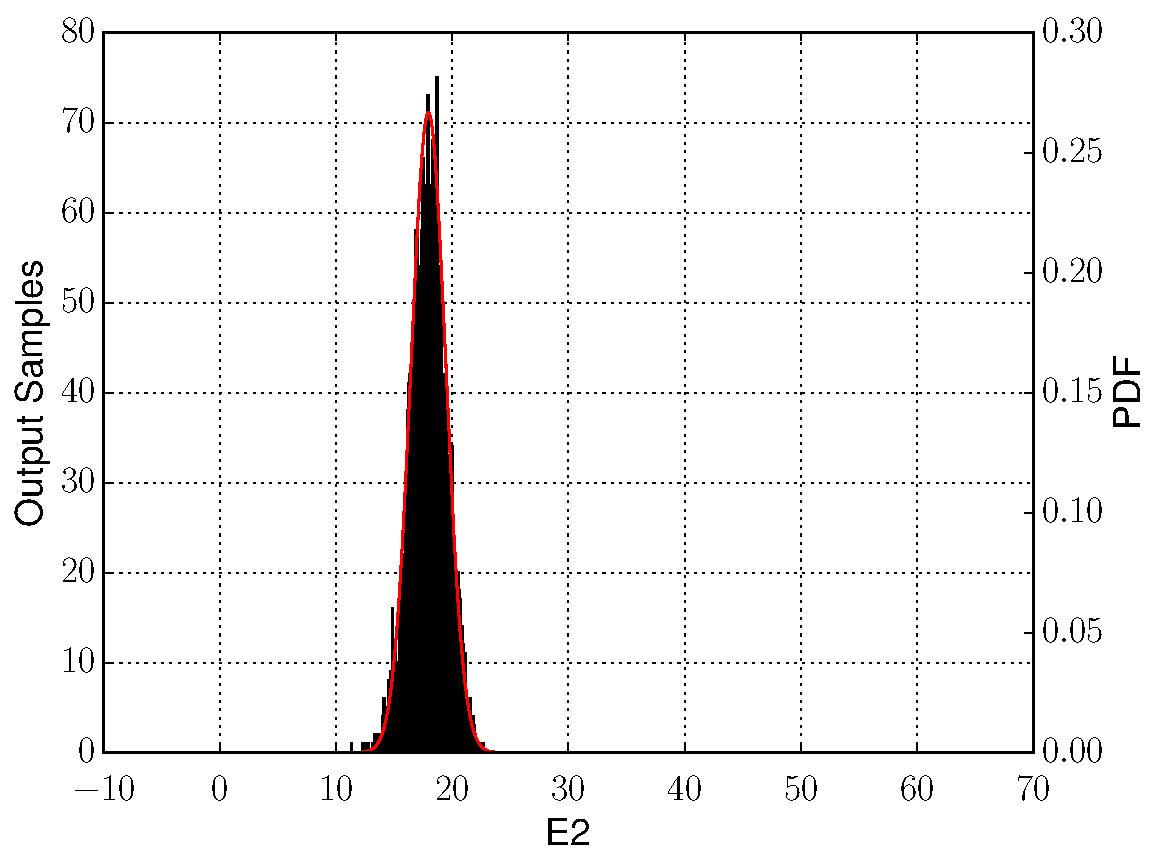
\includegraphics[scale=0.7]{multiple_data/10_kde/outputData_1e5/E2.pdf} 
      }
   \quad
    \subfloat[Histogram for $E_3$ \label{subfig-1:dummy}]{%
          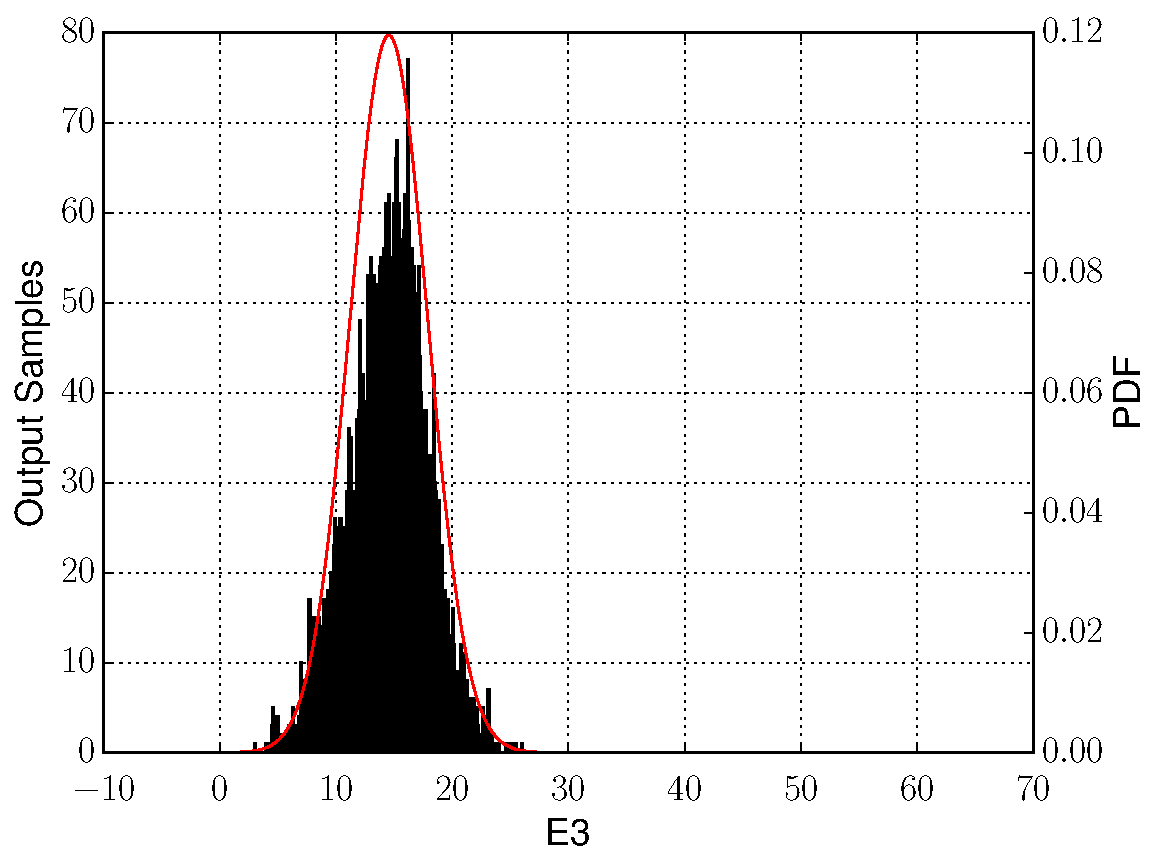
\includegraphics[scale=0.7]{multiple_data/10_kde/outputData_1e5/E3.pdf} 
         }
\end{figure}
\begin{figure}[H]
  
   \subfloat[Cummulative Density Funtion \label{subfig-1:dummy}]{
        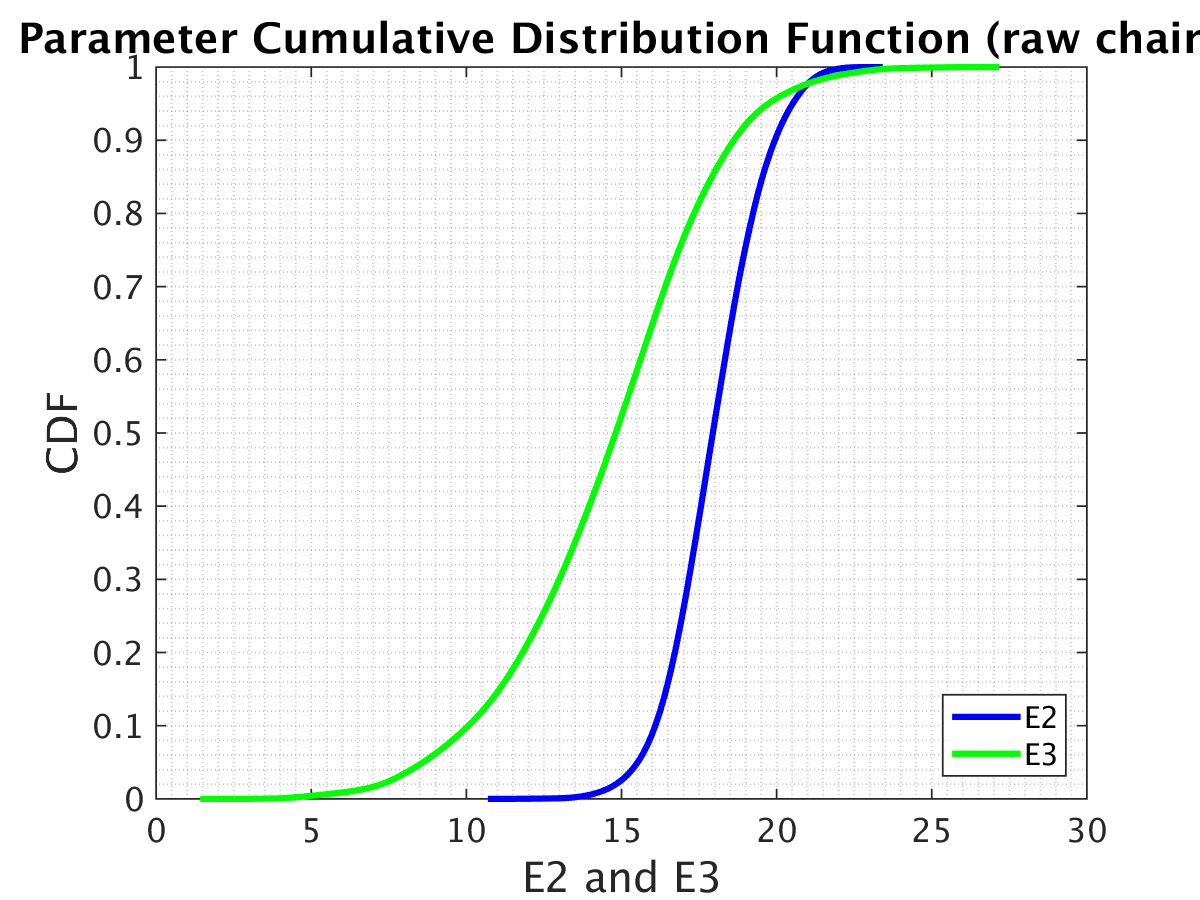
\includegraphics[scale=0.7]{multiple_data/10_kde/outputData_1e5/cdf} 
       }
     \quad
\subfloat[KDE \label{subfig-1:dummy}]{
        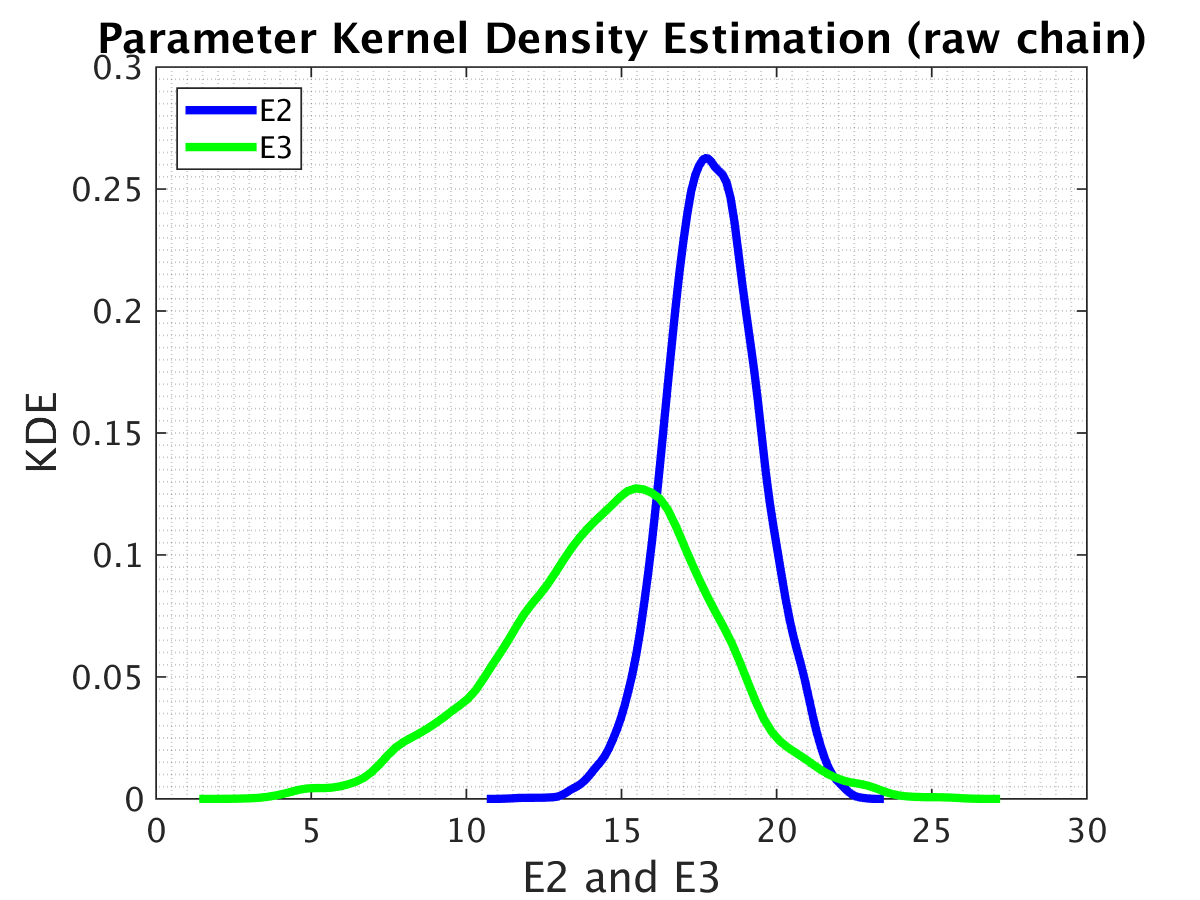
\includegraphics[scale=0.7]{multiple_data/10_kde/outputData_1e5/kde} 
            }  
  \caption{Results for sample size 1e5}
\end{figure}

\begin{figure}[H]
\centering
\subfloat[MCMC raw chain of samples of $E_2$\label{subfig-1:dummy}]{%
     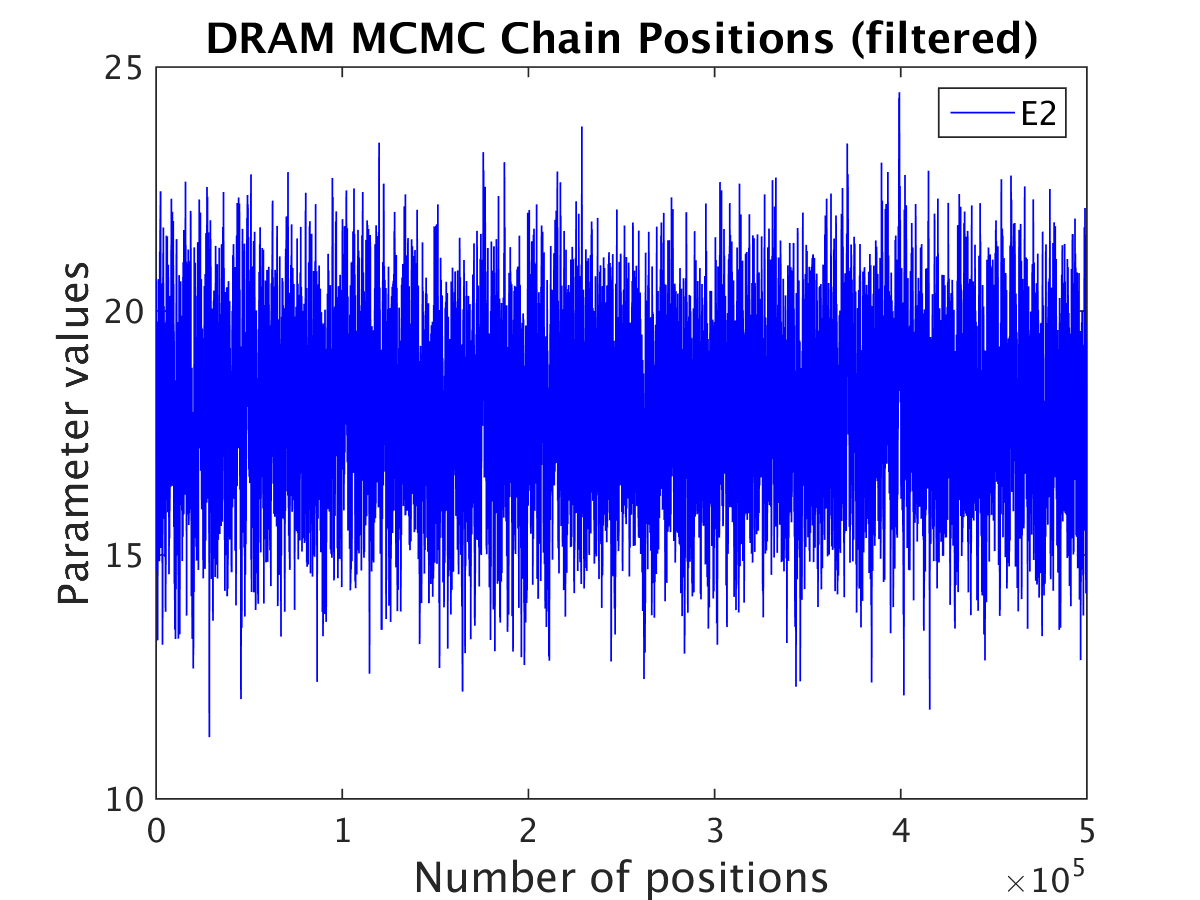
\includegraphics[scale=0.7]{multiple_data/10_kde/outputData_5e5/simple_ip_chain_pos_raw_1} 
    }
    \quad
    \subfloat[MCMC raw chain of samples of $E_2$\label{subfig-1:dummy}]{%
         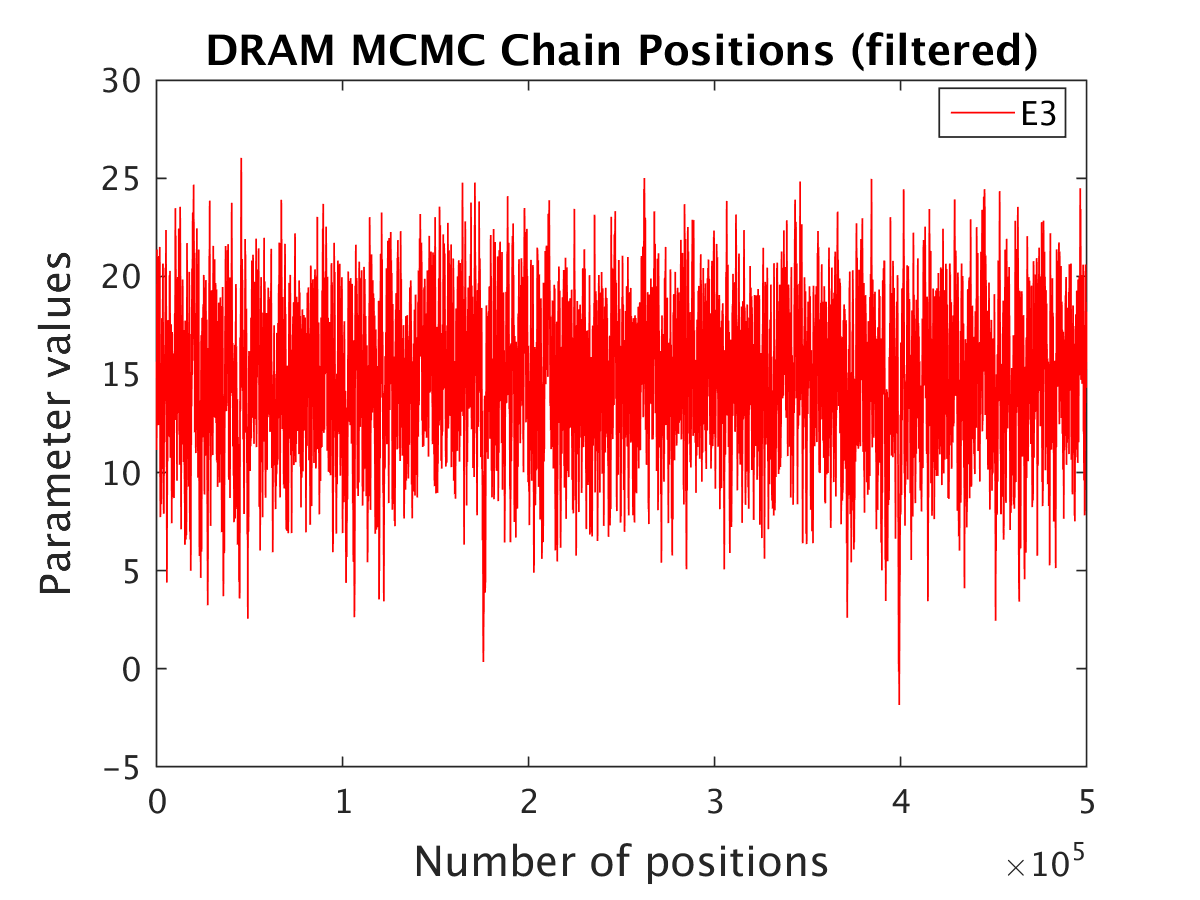
\includegraphics[scale=0.7]{multiple_data/10_kde/outputData_5e5/simple_ip_chain_pos_raw_2} 
        }
    \end{figure}
  \begin{figure}[H]
  \ContinuedFloat
  \centering
  \subfloat[Histogram for $E_2$ \label{subfig-1:dummy}]{%
       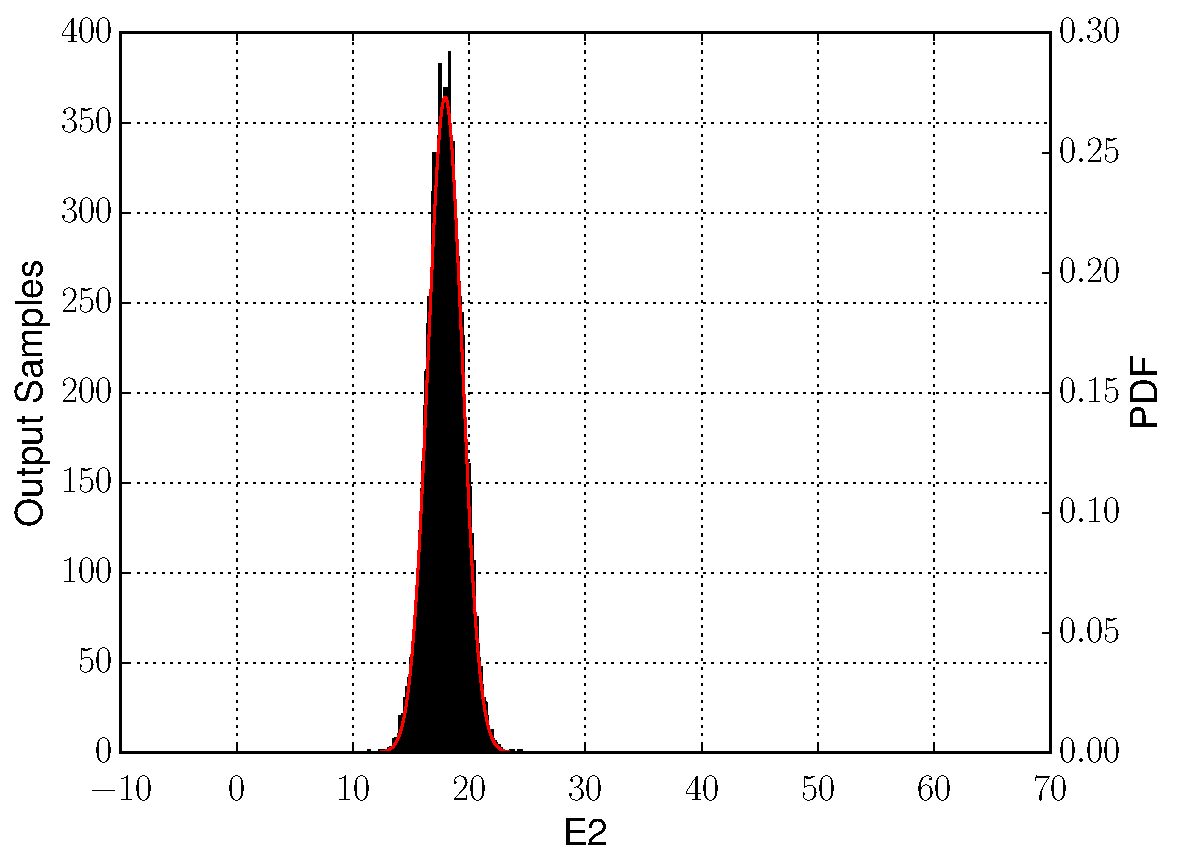
\includegraphics[scale=0.7]{multiple_data/10_kde/outputData_5e5/E2.pdf} 
      }
   \quad
    \subfloat[Histogram for $E_3$ \label{subfig-1:dummy}]{%
          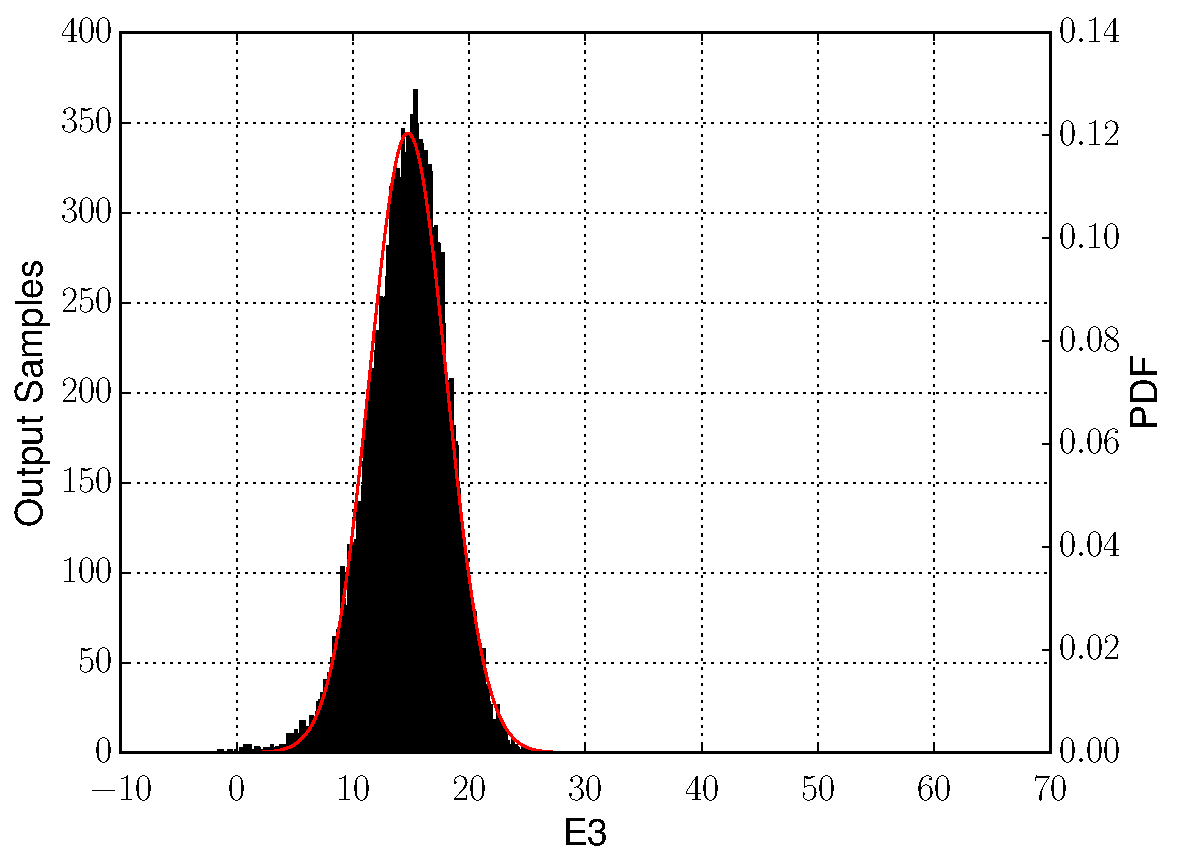
\includegraphics[scale=0.7]{multiple_data/10_kde/outputData_5e5/E3.pdf} 
         }
\end{figure}
\begin{figure}[H]
  
   \subfloat[Cummulative Density Funtion \label{subfig-1:dummy}]{
        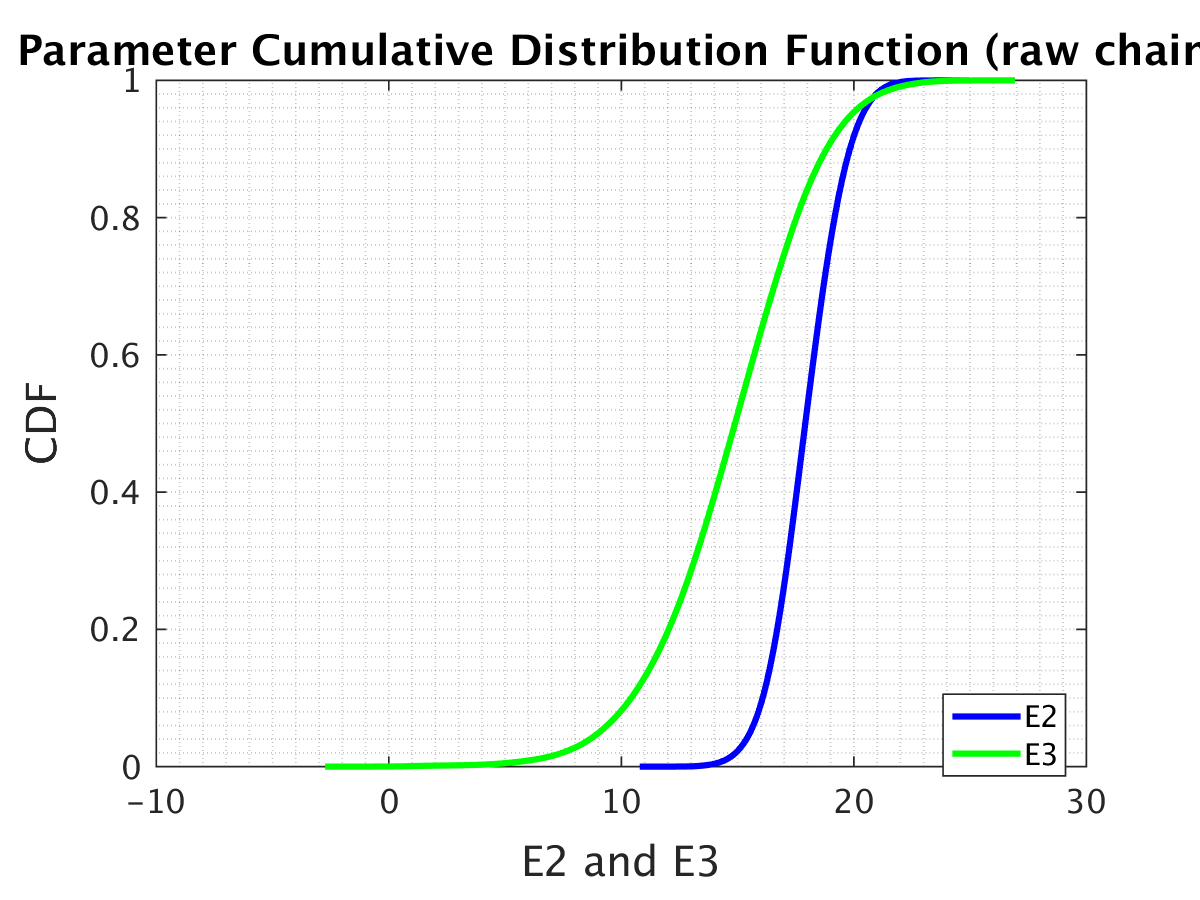
\includegraphics[scale=0.7]{multiple_data/10_kde/outputData_5e5/cdf} 
       }
     \quad
\subfloat[KDE \label{subfig-1:dummy}]{
        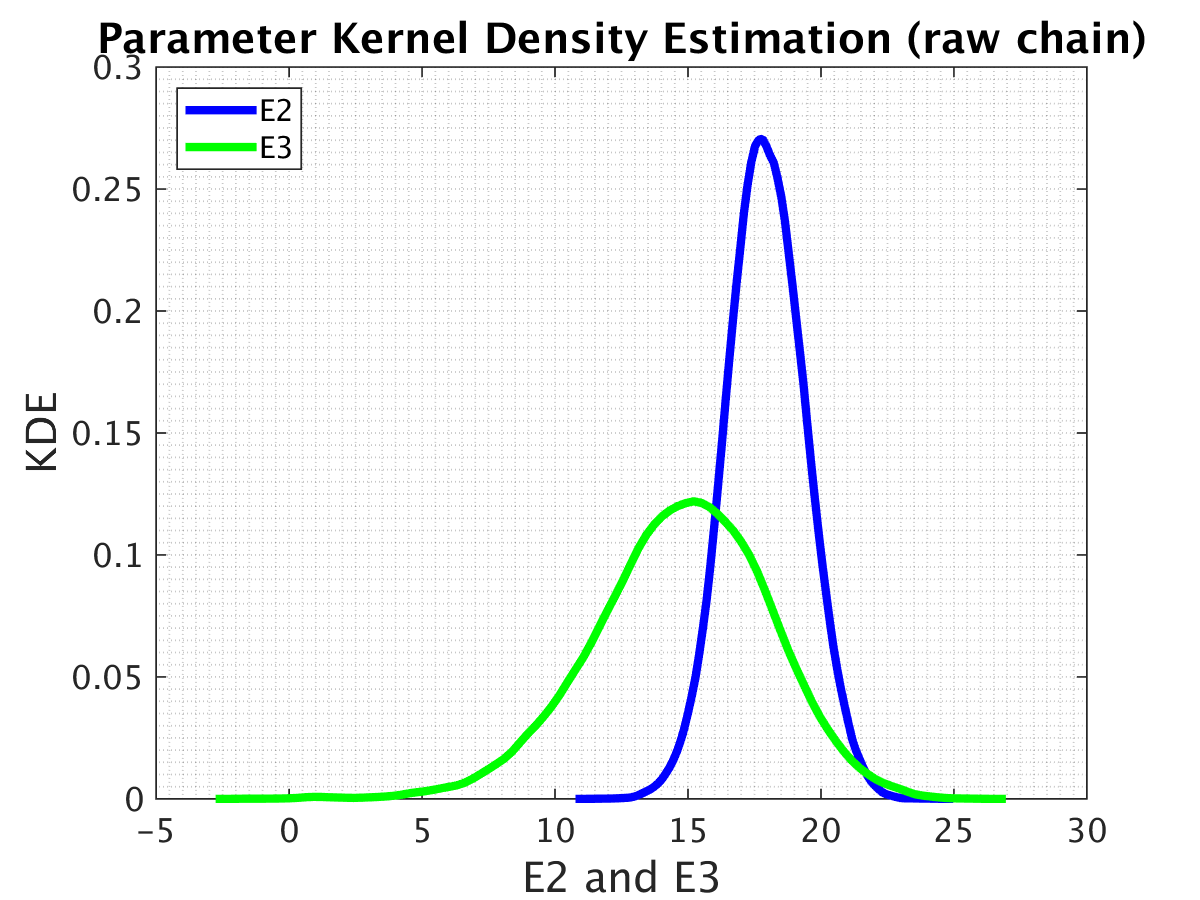
\includegraphics[scale=0.7]{multiple_data/10_kde/outputData_5e5/kde} 
            }  
  \caption{Results for sample size 5e5}
\end{figure}


\begin{figure}[H]
\centering
\subfloat[MCMC raw chain of samples of $E_2$\label{subfig-1:dummy}]{%
     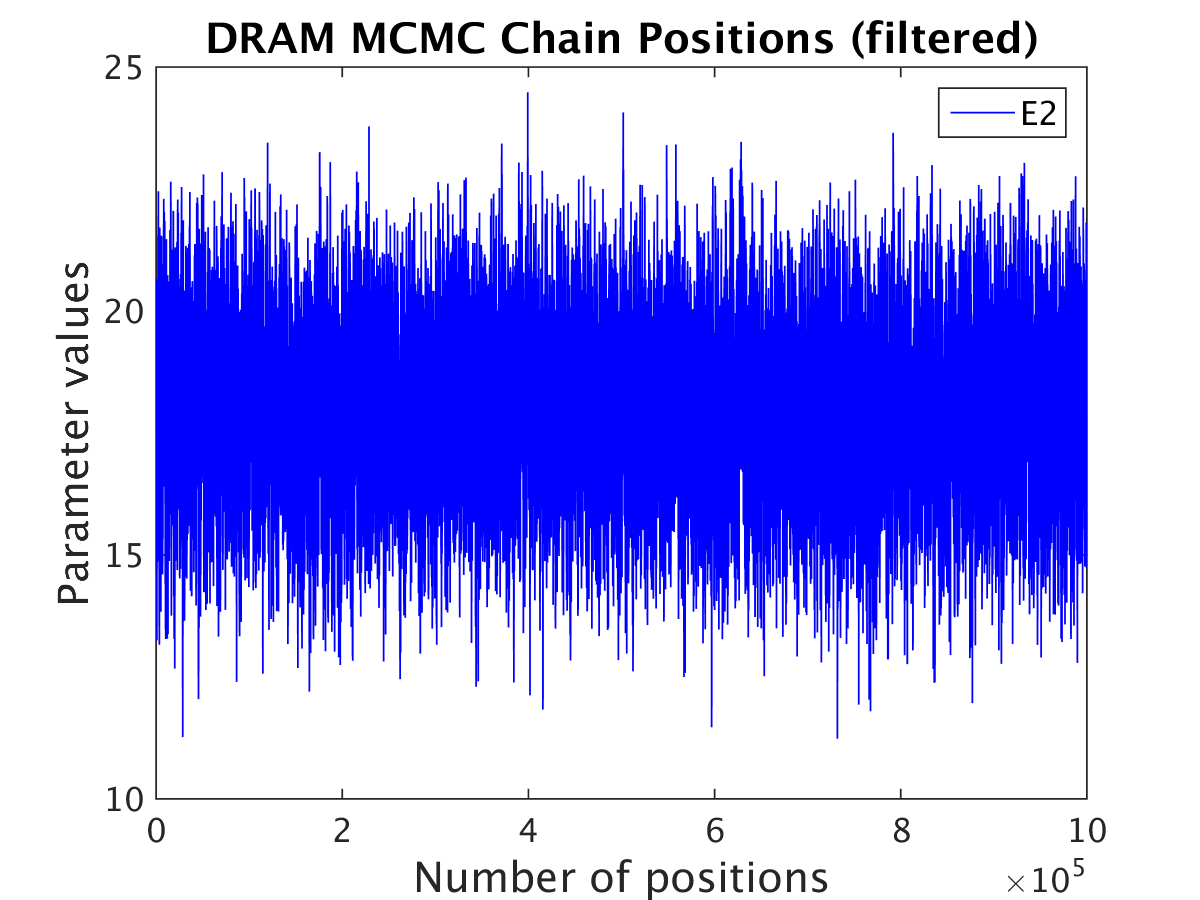
\includegraphics[scale=0.7]{multiple_data/10_kde/outputData_1e6/simple_ip_chain_pos_raw_1} 
    }
    \quad
    \subfloat[MCMC raw chain of samples of $E_2$\label{subfig-1:dummy}]{%
         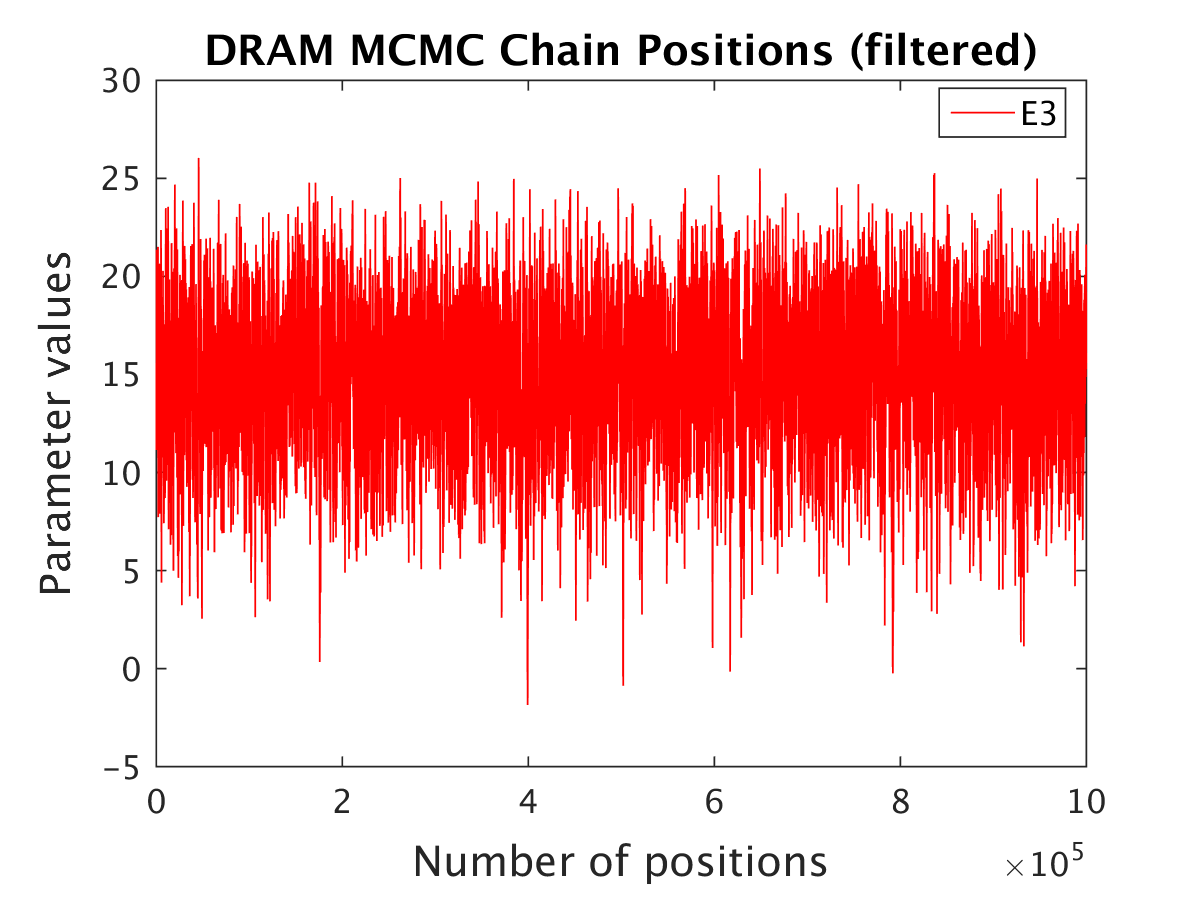
\includegraphics[scale=0.7]{multiple_data/10_kde/outputData_1e6/simple_ip_chain_pos_raw_2} 
        }
    \end{figure}
  \begin{figure}[H]
  \ContinuedFloat
  \centering
  \subfloat[Histogram for $E_2$ \label{subfig-1:dummy}]{%
       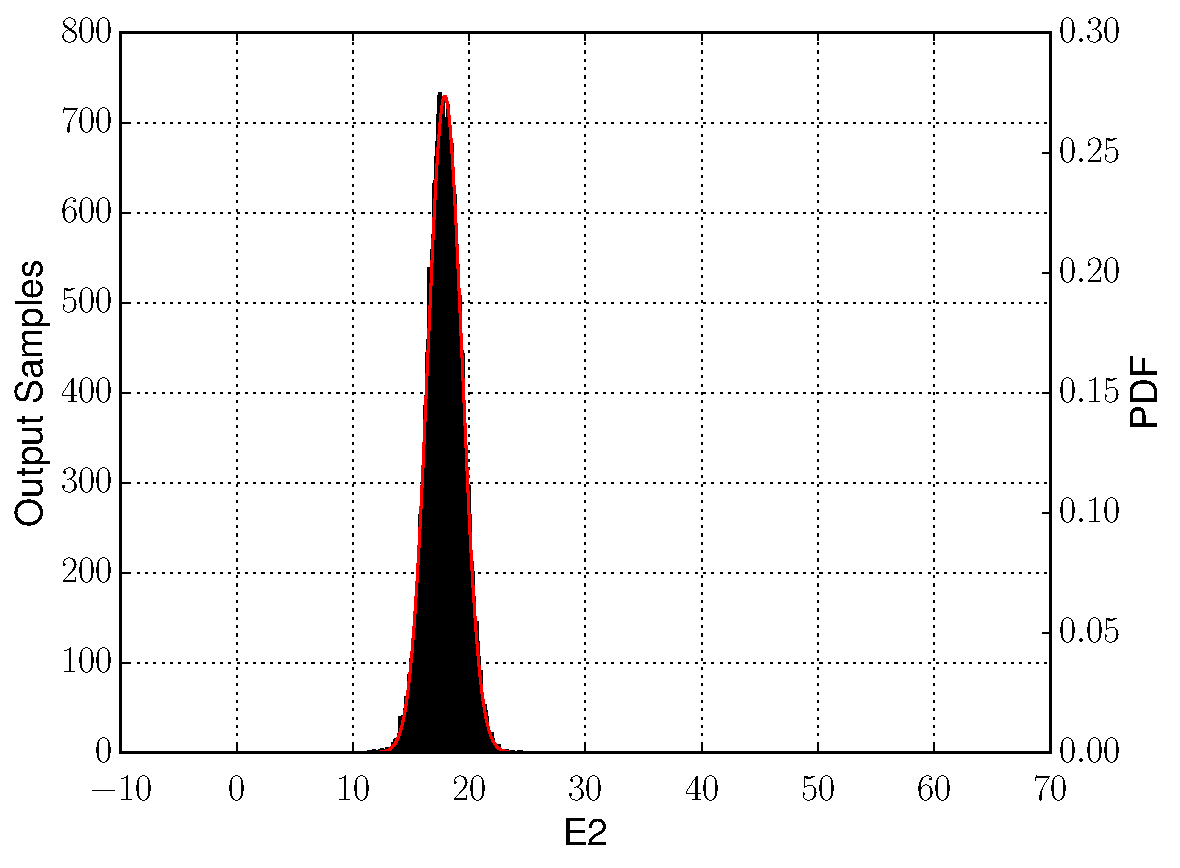
\includegraphics[scale=0.7]{multiple_data/10_kde/outputData_1e6/E2.pdf} 
      }
   \quad
    \subfloat[Histogram for $E_3$ \label{subfig-1:dummy}]{%
          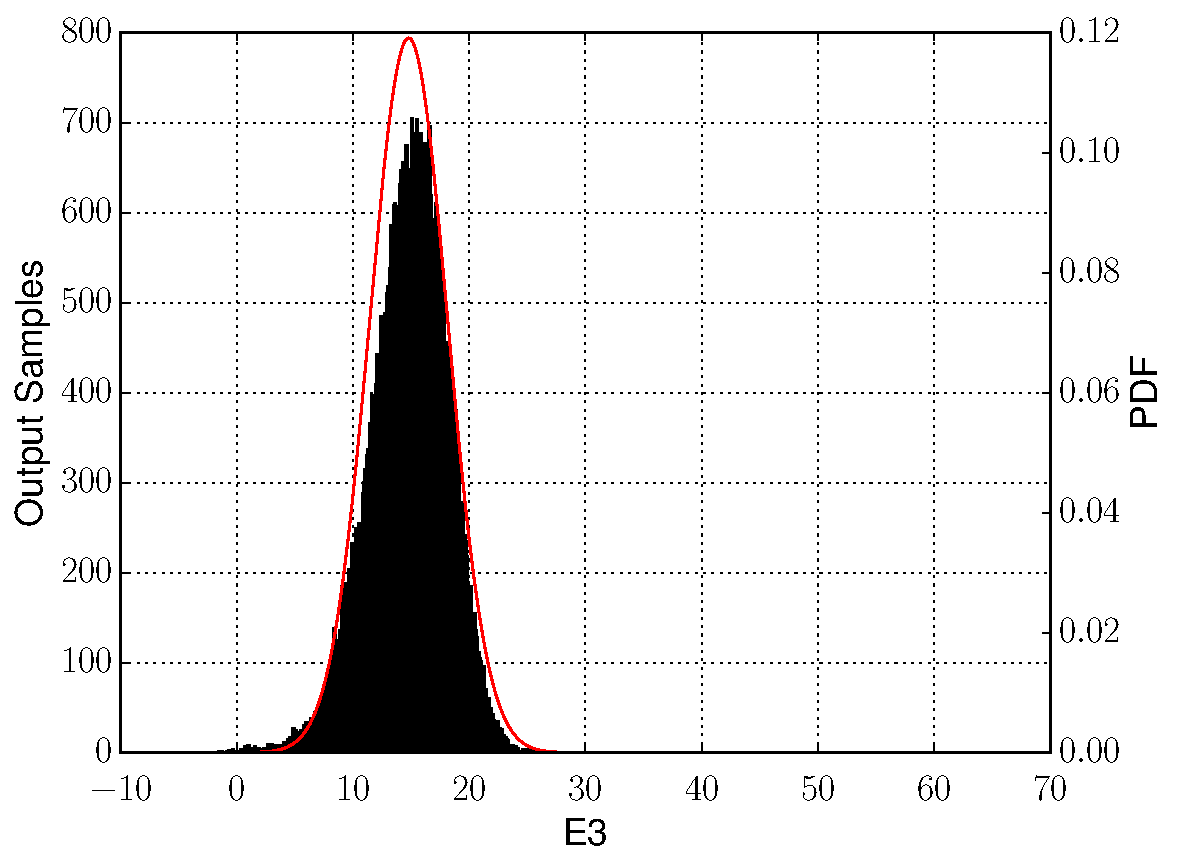
\includegraphics[scale=0.7]{multiple_data/10_kde/outputData_1e6/E3.pdf} 
         }
\end{figure}
\begin{figure}[H]
  
   \subfloat[Cummulative Density Funtion \label{subfig-1:dummy}]{
        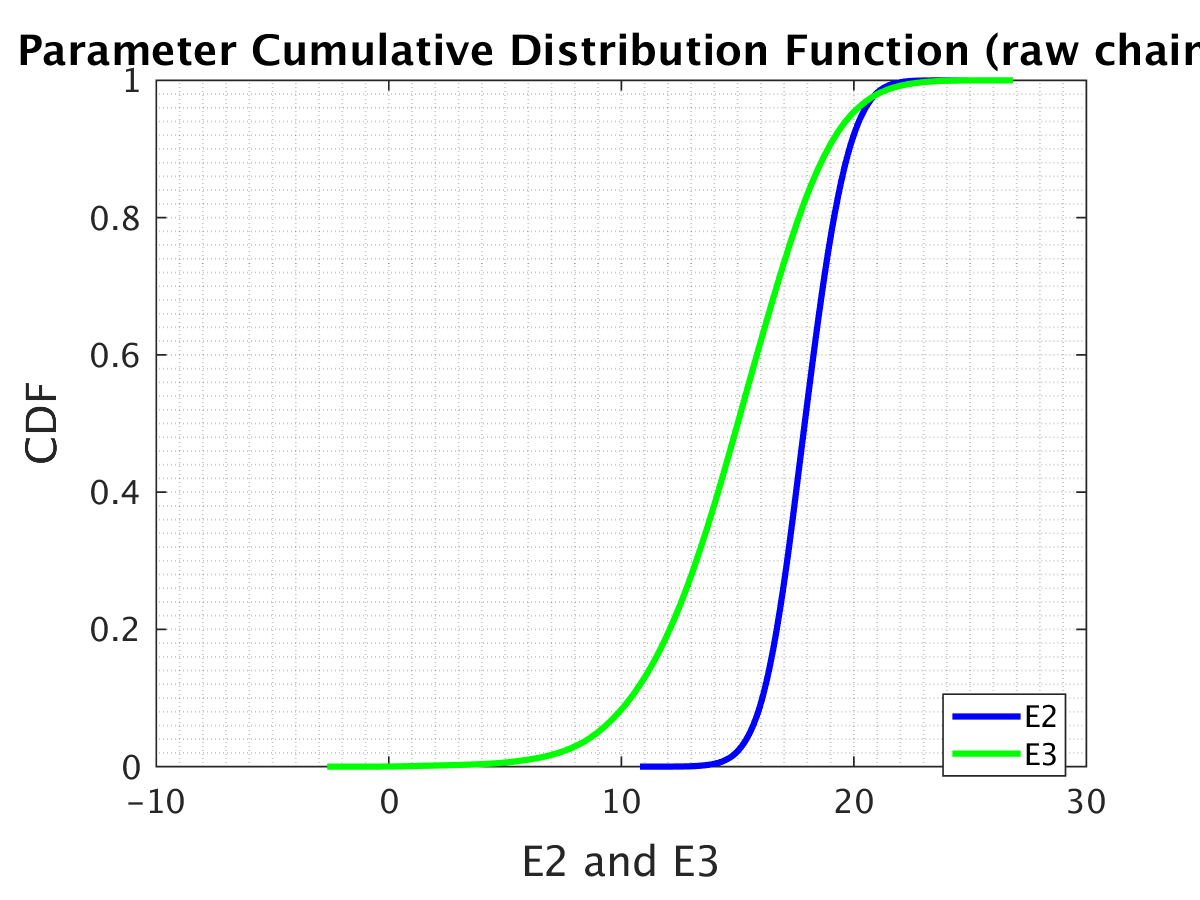
\includegraphics[scale=0.7]{multiple_data/10_kde/outputData_1e6/cdf} 
       }
     \quad
\subfloat[KDE \label{subfig-1:dummy}]{
        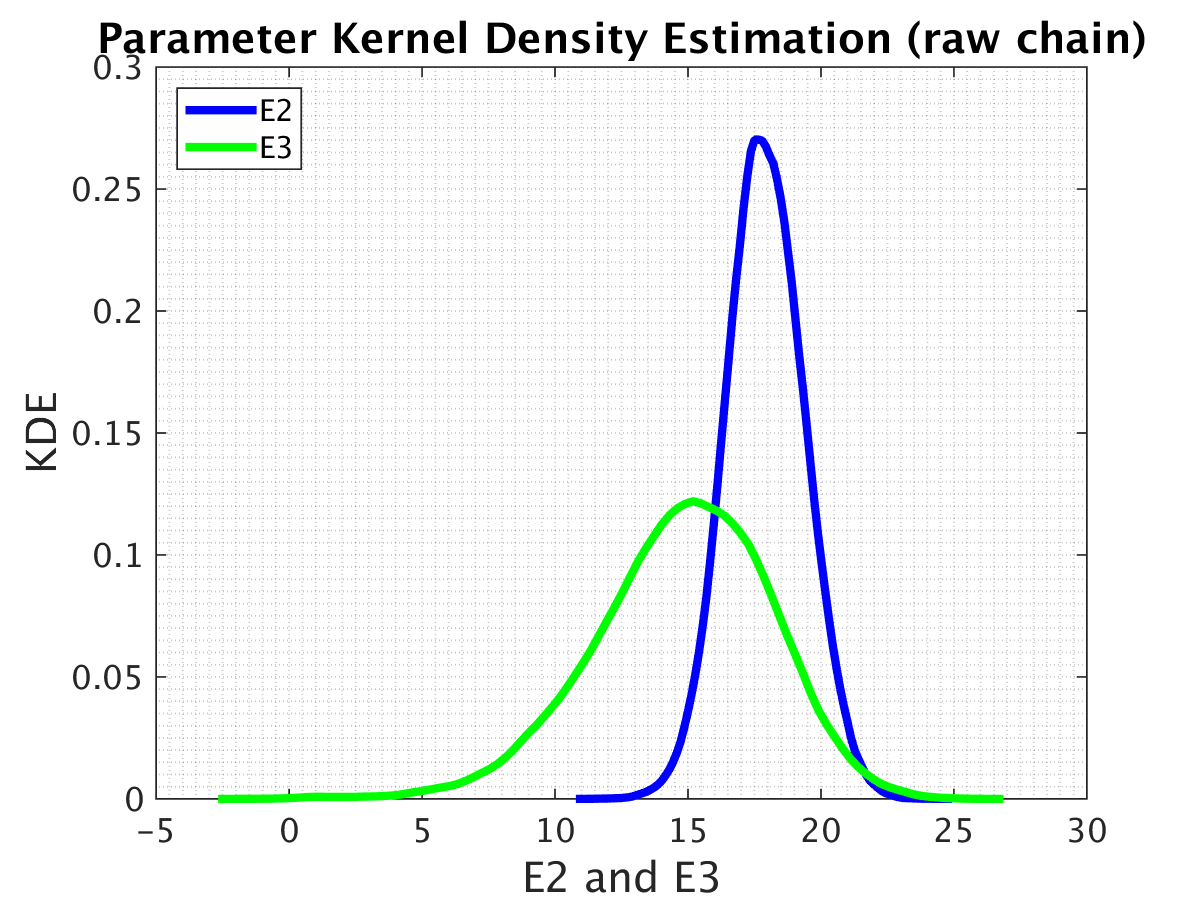
\includegraphics[scale=0.7]{multiple_data/10_kde/outputData_1e6/kde} 
            }  
  \caption{Results for sample size 1e6}
\end{figure}


\begin{figure}[H]
\centering
\subfloat[MCMC raw chain of samples of $E_2$\label{subfig-1:dummy}]{%
     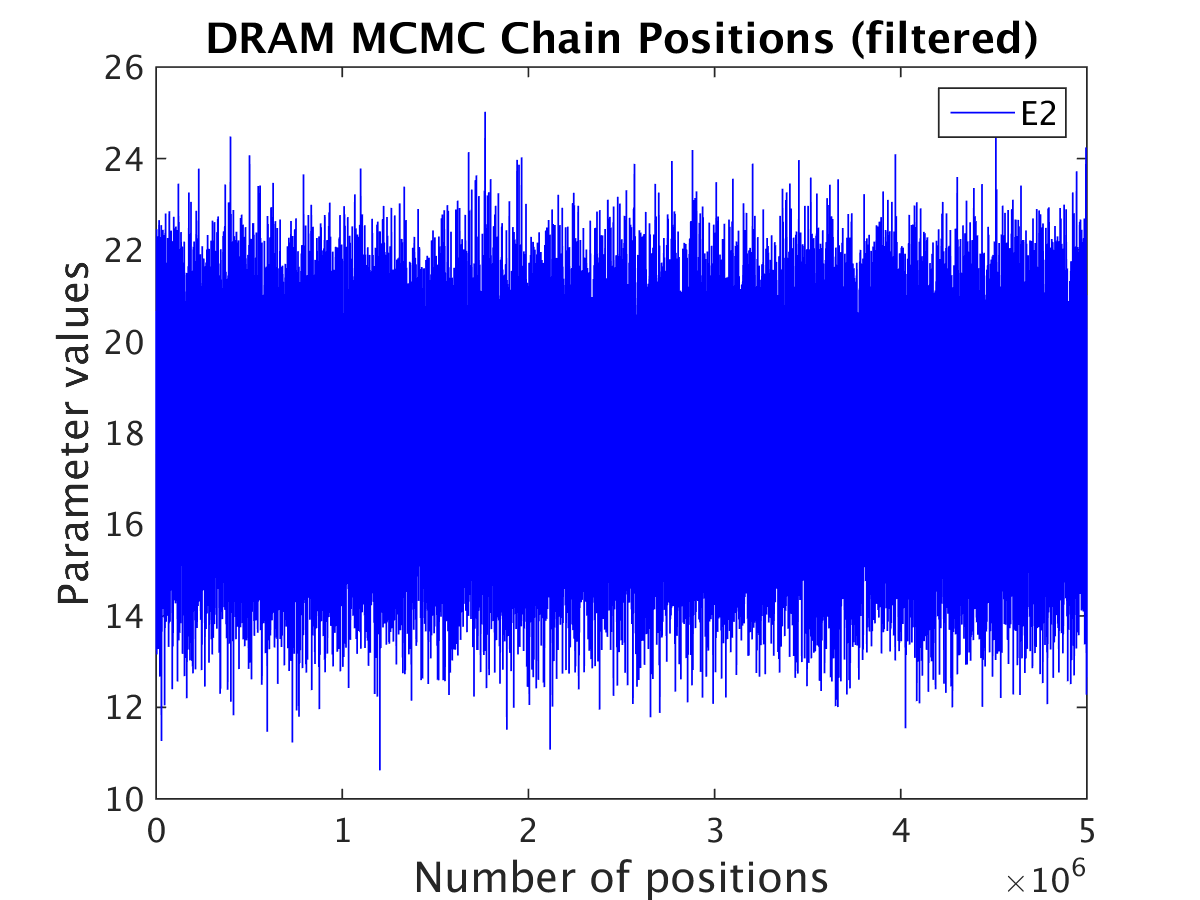
\includegraphics[scale=0.7]{multiple_data/10_kde/outputData_5e6/simple_ip_chain_pos_raw_1} 
    }
    \quad
    \subfloat[MCMC raw chain of samples of $E_2$\label{subfig-1:dummy}]{%
         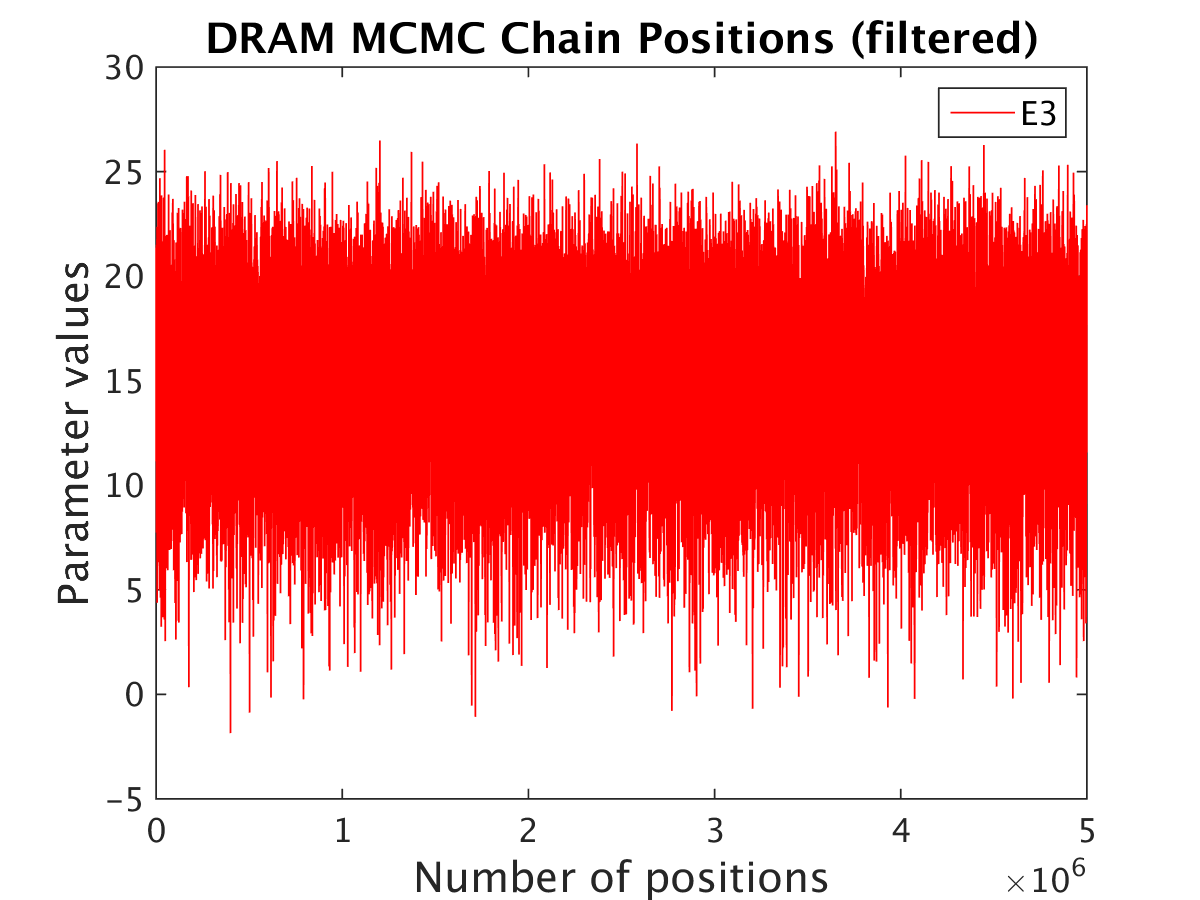
\includegraphics[scale=0.7]{multiple_data/10_kde/outputData_5e6/simple_ip_chain_pos_raw_2} 
        }
    \end{figure}
  \begin{figure}[H]
  \ContinuedFloat
  \centering
  \subfloat[Histogram for $E_2$ \label{subfig-1:dummy}]{%
       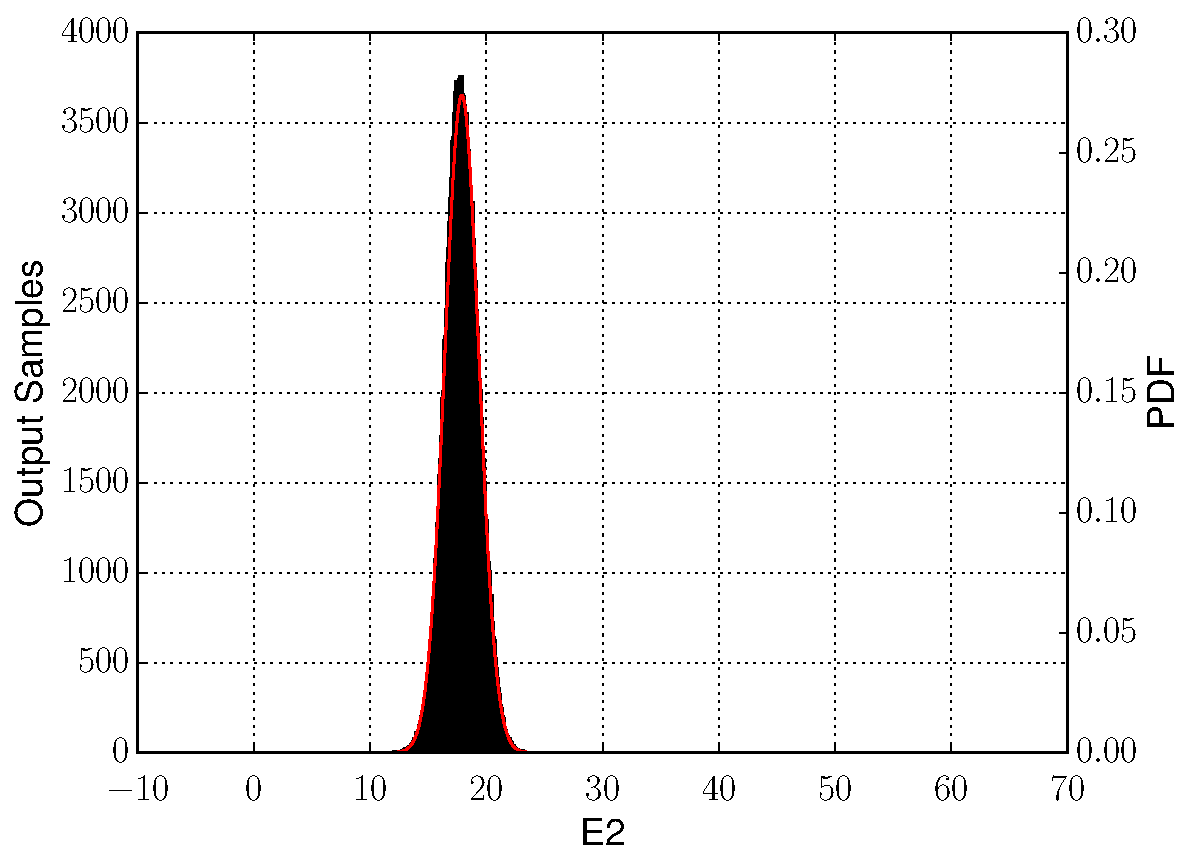
\includegraphics[scale=0.7]{multiple_data/10_kde/outputData_5e6/E2.pdf} 
      }
   \quad
    \subfloat[Histogram for $E_3$ \label{subfig-1:dummy}]{%
          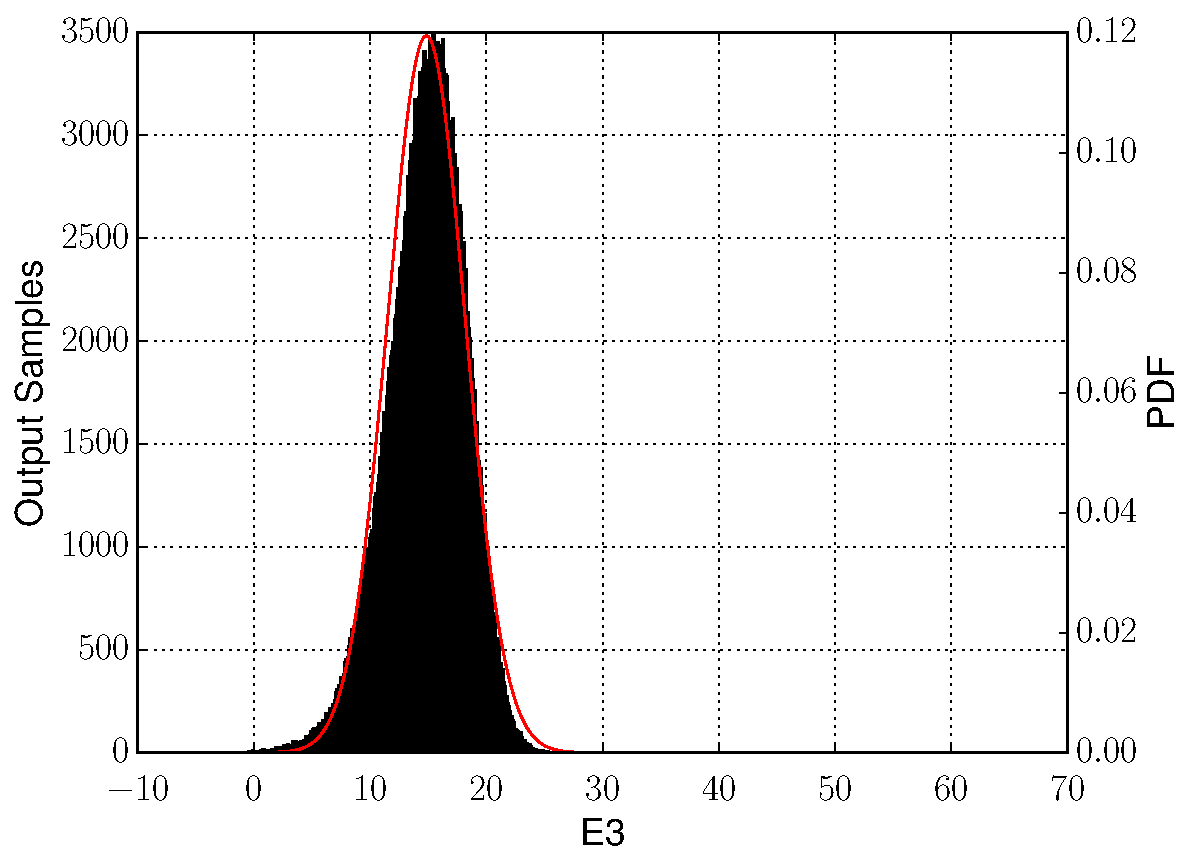
\includegraphics[scale=0.7]{multiple_data/10_kde/outputData_5e6/E3.pdf} 
         }
\end{figure}
\begin{figure}[H]
  
   \subfloat[Cummulative Density Funtion \label{subfig-1:dummy}]{
        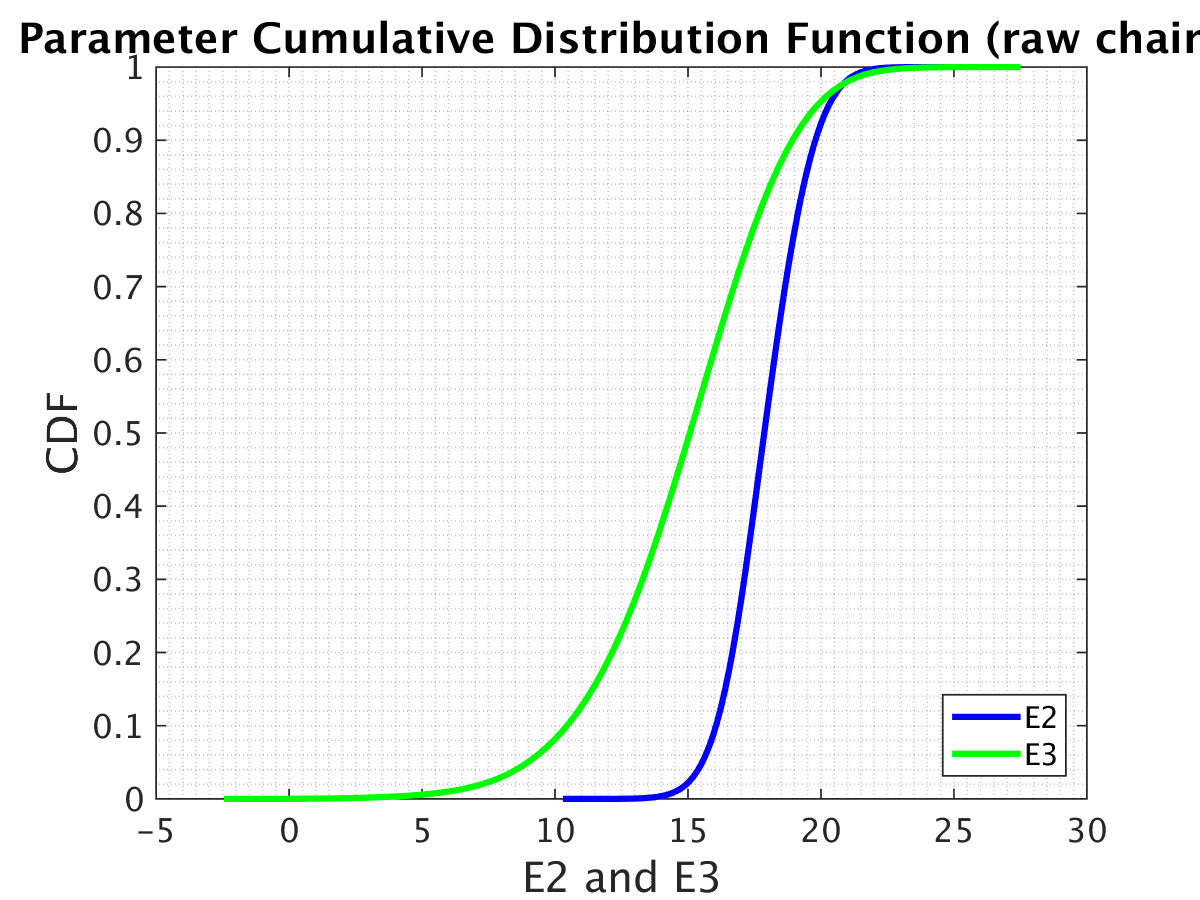
\includegraphics[scale=0.7]{multiple_data/10_kde/outputData_5e6/cdf} 
       }
     \quad
\subfloat[KDE \label{subfig-1:dummy}]{
        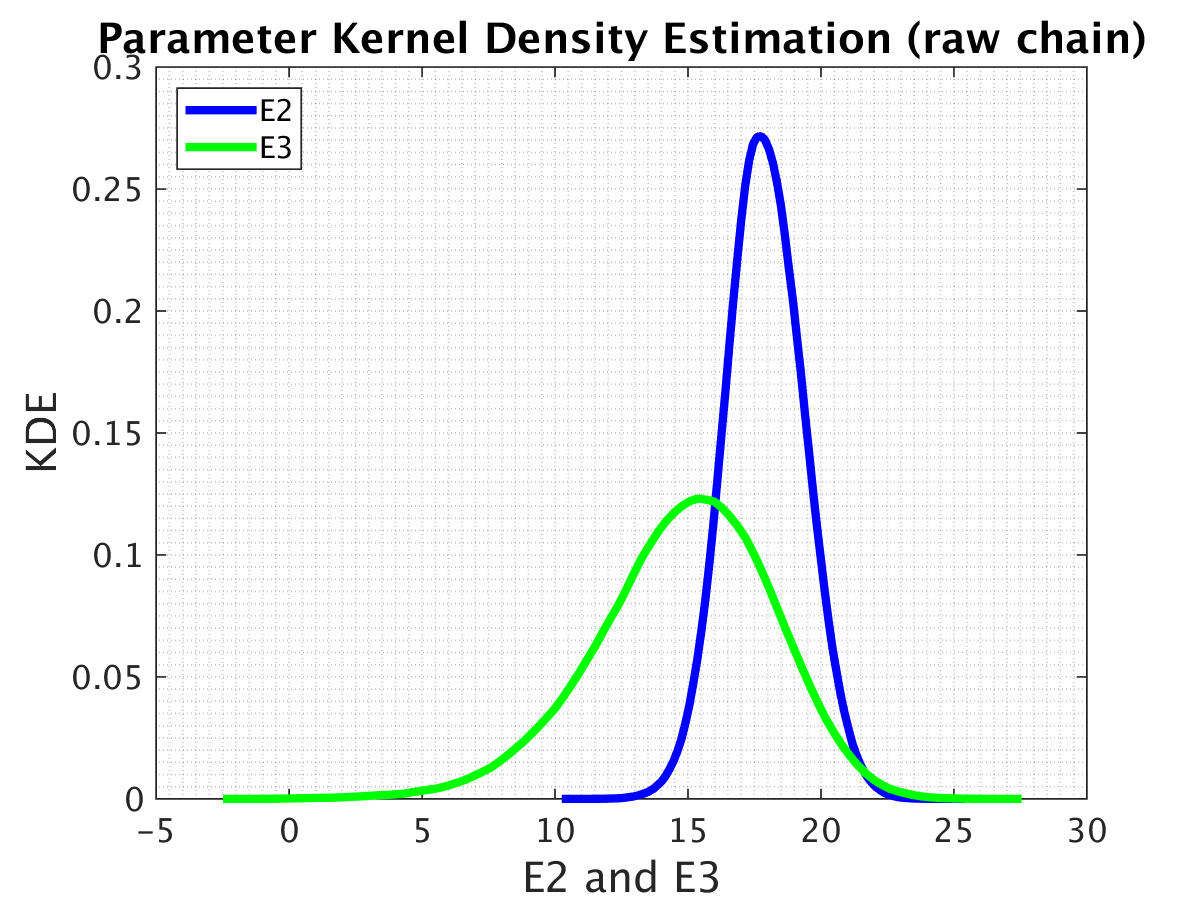
\includegraphics[scale=0.7]{multiple_data/10_kde/outputData_5e6/kde} 
            }  
  \caption{Results for sample size 5e6}
\end{figure}

\begin{figure}[H]
\centering
\subfloat[MCMC raw chain of samples of $E_2$\label{subfig-1:dummy}]{%
     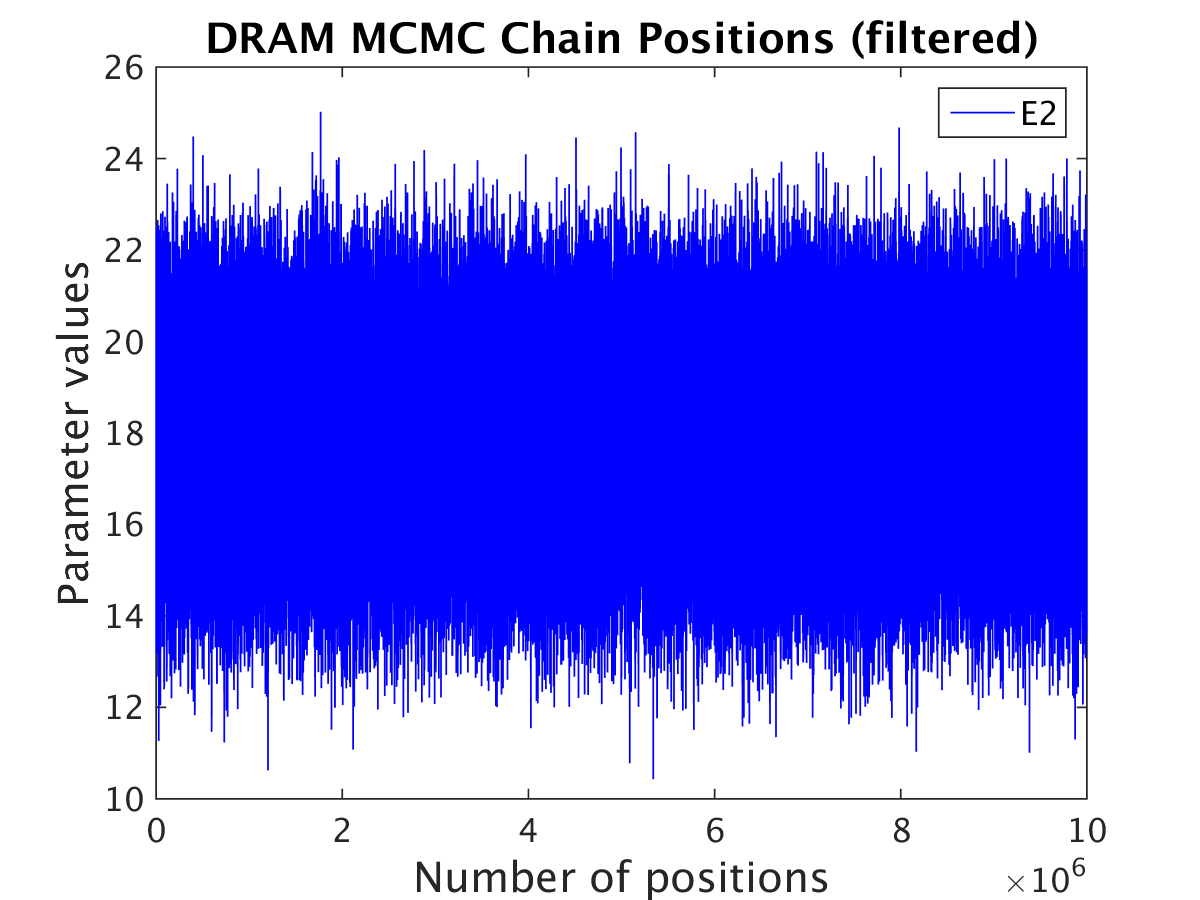
\includegraphics[scale=0.7]{multiple_data/10_kde/outputData_1e7/simple_ip_chain_pos_raw_1} 
    }
    \quad
    \subfloat[MCMC raw chain of samples of $E_2$\label{subfig-1:dummy}]{%
         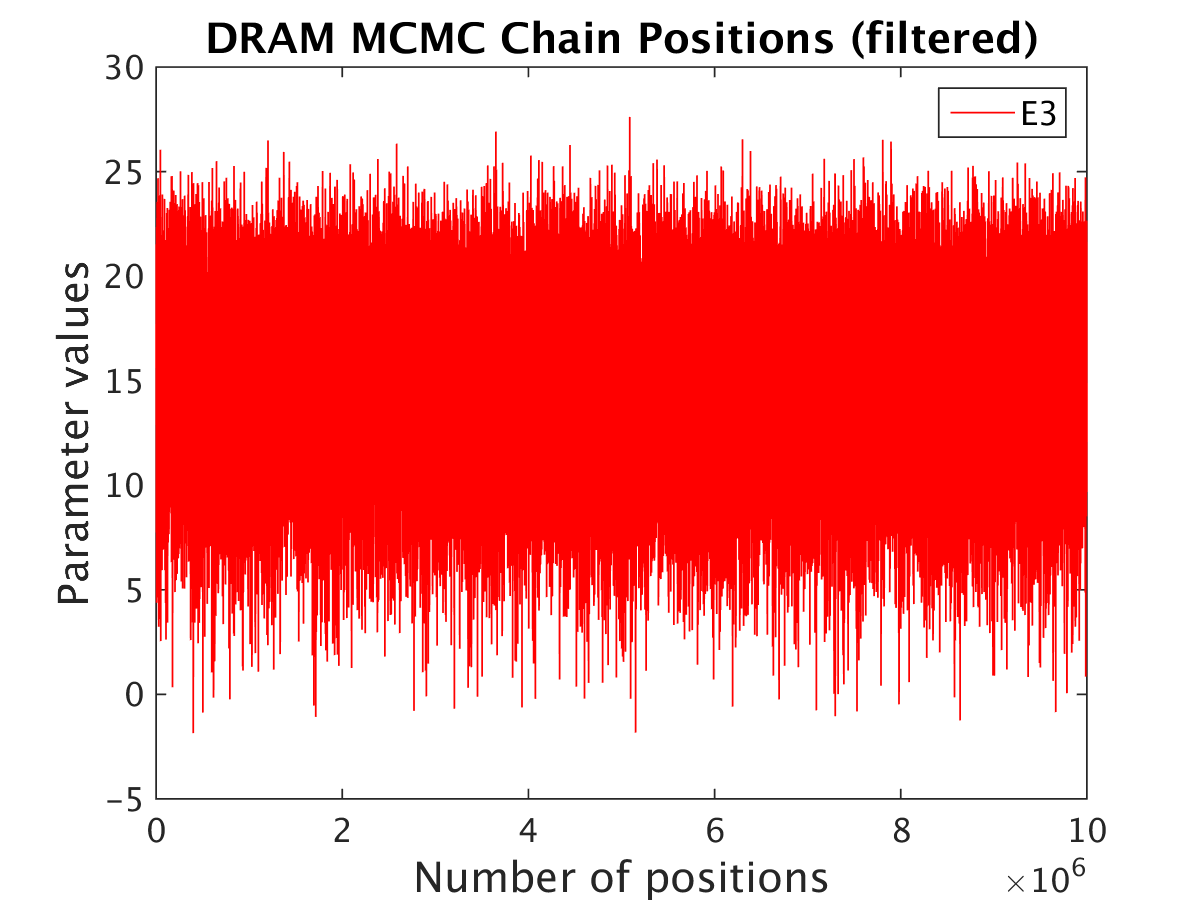
\includegraphics[scale=0.7]{multiple_data/10_kde/outputData_1e7/simple_ip_chain_pos_raw_2} 
        }
    \end{figure}
  \begin{figure}[H]
  \ContinuedFloat
  \centering
  \subfloat[Histogram for $E_2$ \label{subfig-1:dummy}]{%
       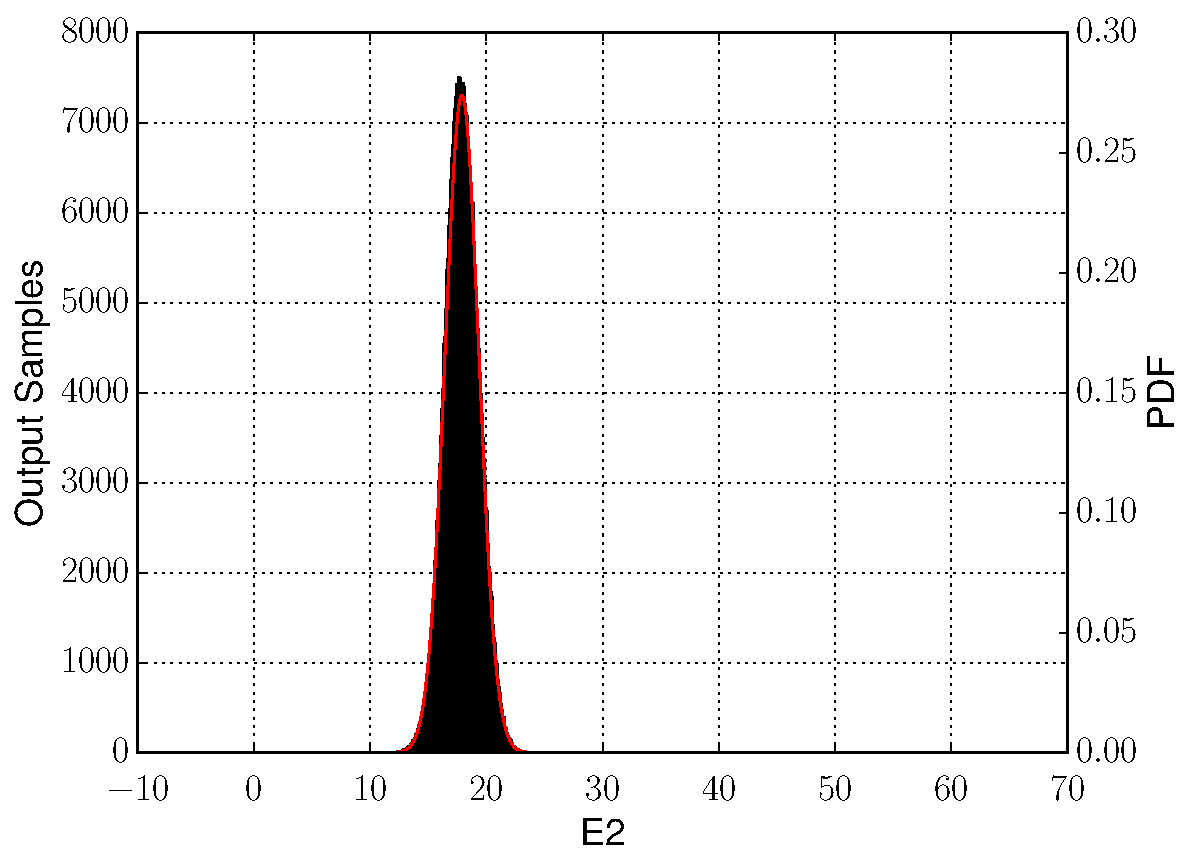
\includegraphics[scale=0.7]{multiple_data/10_kde/outputData_1e7/E2.pdf} 
      }
   \quad
    \subfloat[Histogram for $E_3$ \label{subfig-1:dummy}]{%
          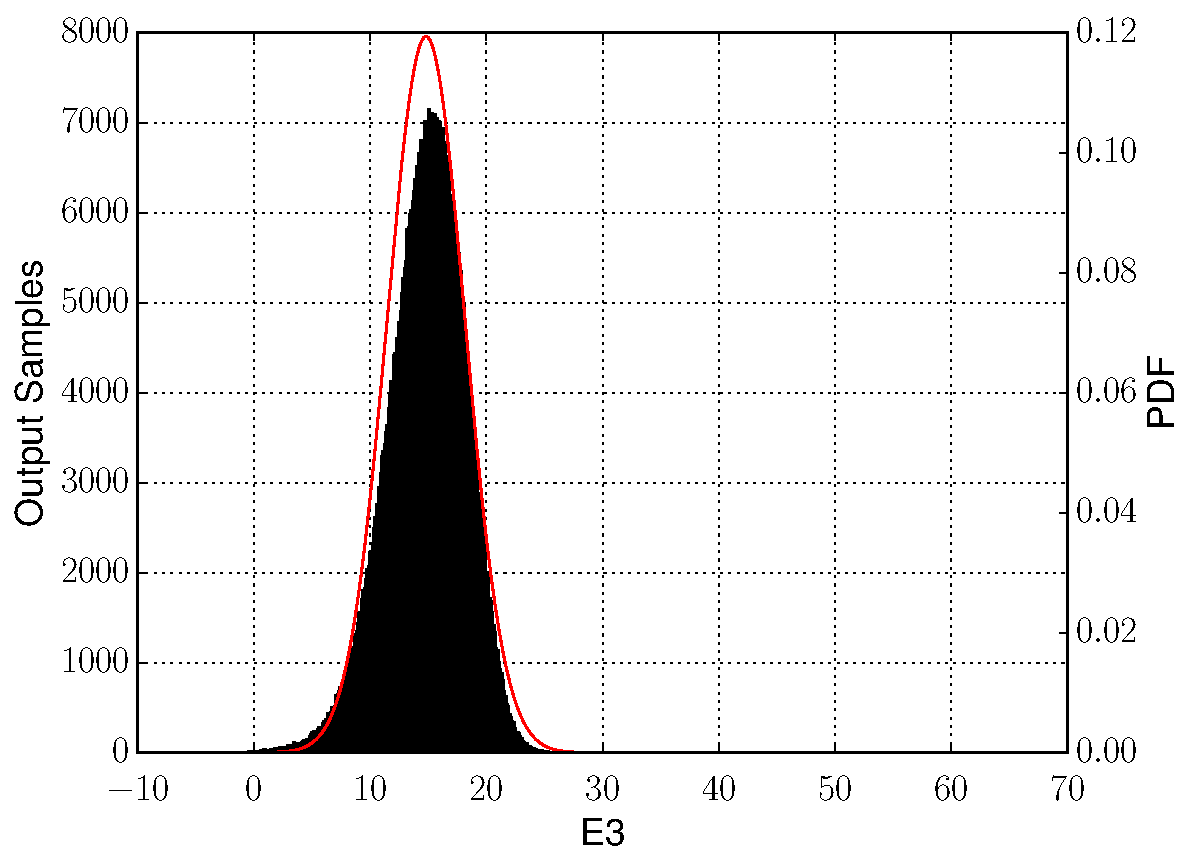
\includegraphics[scale=0.7]{multiple_data/10_kde/outputData_1e7/E3.pdf} 
         }
\end{figure}
\begin{figure}[H]
  
   \subfloat[Cummulative Density Funtion \label{subfig-1:dummy}]{
        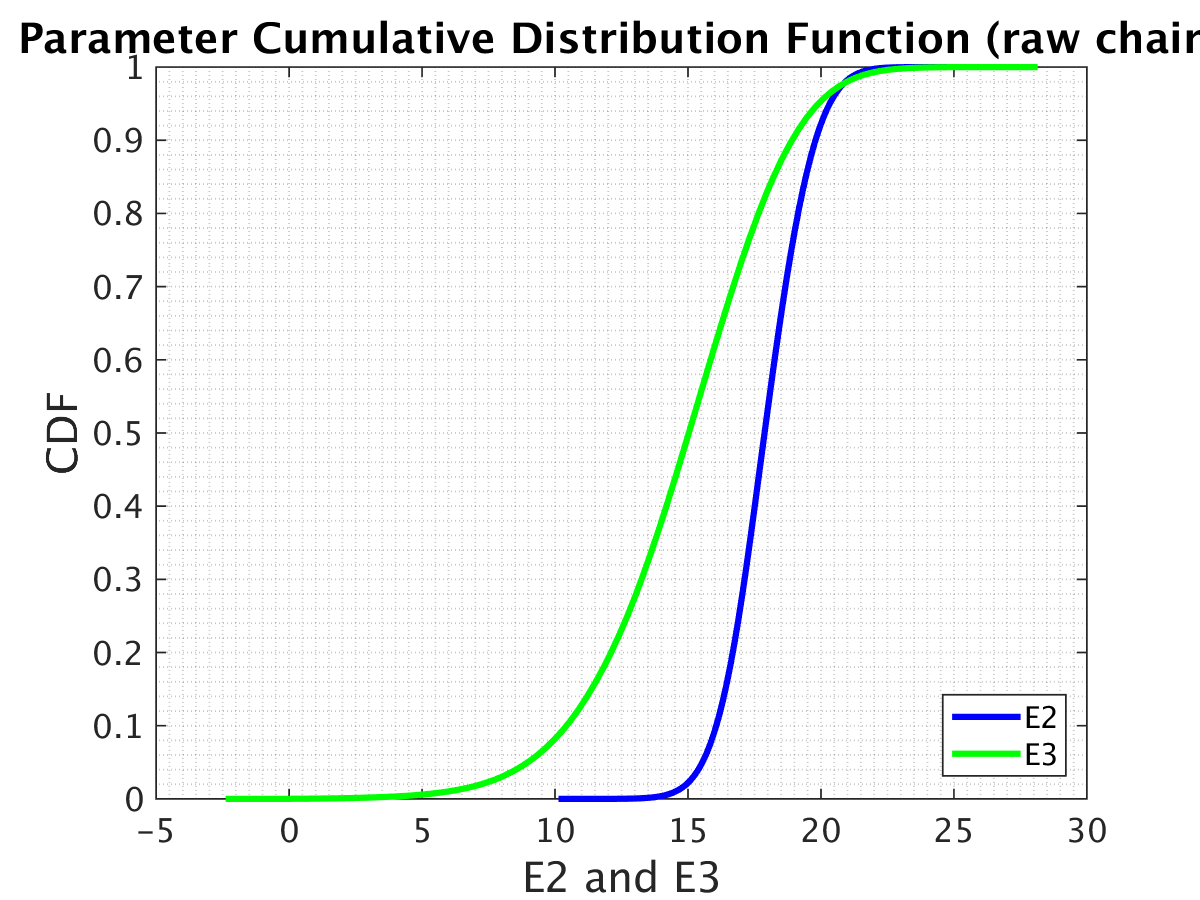
\includegraphics[scale=0.7]{multiple_data/10_kde/outputData_1e7/cdf} 
       }
     \quad
\subfloat[KDE \label{subfig-1:dummy}]{
        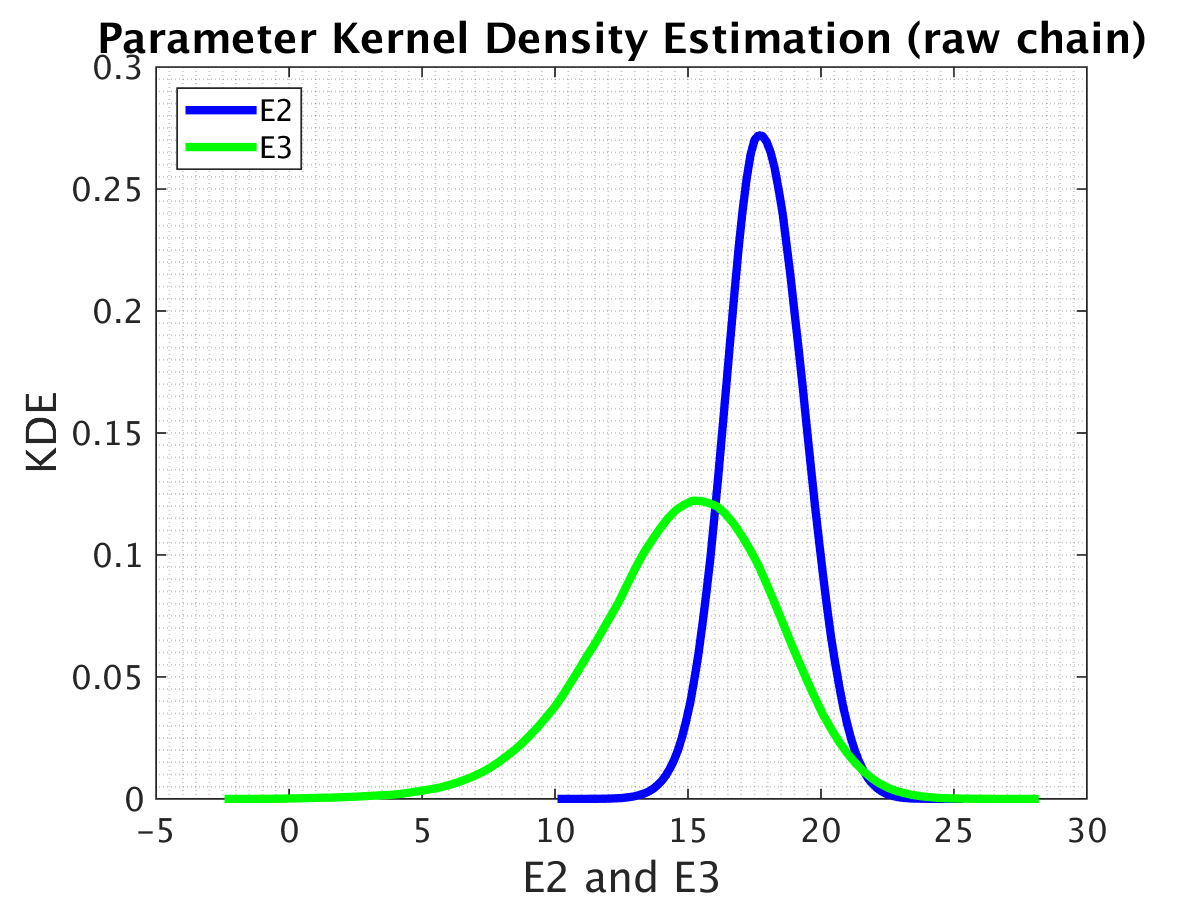
\includegraphics[scale=0.7]{multiple_data/10_kde/outputData_1e7/kde} 
            }  
  \caption{Results for sample size 1e7}
\end{figure}